\chapter{Dokumentaja techniczna}\label{chap:dokumentacja-techniczna}
Niniejszy rozdział stanowi objaśnienie, w jaki sposób system został stworzony. Zawiera opis wymagań oraz szczegóły implementacyjne dotyczące budowy poszczególnych warstw przy wykorzystaniu technologii opisanych w rozdziale \ref{chap:zastosowane-technologie}.
\section{Projekt systemu}
\subsection{Opis założeń}
moja-aplikacja składa się z aplikacji przeznaczonej na urządzenia z systemem Android \cite{android} oraz wspierającej ją aplikacji webowej. Komunikacja pomiędzy nimi odbywa się poprzez protokół HTTP (\textit{Hypertext Transfer Protocol}), a sam interfejs aplikacji serwerowej został wykonany w stylu \textbf{REST} (\textit{Representational state transfer}). Oznacza to między innymi, że konkretny zasób na serwerze jest identyfikowany na podstawie przypisanego mu URI (\textit{Uniform Resource Identifier}), a użytkownik odpytujący serwer jest identyfikowany na podstawie parametru zawartego w nagłówkach żądania. Wymiana danych pomiędzy obiema aplikacjami odbywa się przy pomocy formatu JSON (\textit{JavaScript Object Notation}). \cite{ksiazka-asp-core}

\subsubsection{Aplikacja mobilna powinna:}
\begin{itemize}
\item{Umożliwiać wieloplatformość} - zastosowana architektura powinna oddzielać logikę biznesową aplikacji od interfejsu graficznego. W efekcie dzięki zastosowaniu technologii Xamarin, przeniesienie aplikacji na inny mobilny system operacyjny powinno ograniczać się do zbudowania jedynie widoku przeznaczonego pod ten system.
\item{Udostępniać użytkownikowi interfejs służący do stworzenia konta i uwierzytelnienia się.}
\item{Przed umożliwieniem utworzenia trasy, wyszukania jej lub przeprowadzenia treningu wymagać uwierzytelnienia się w systemie.}
\item{Pozwalać użytkownikom tworzyć trasy, a także umożliwiać manualne lub automatyczne określenie ich cech.}
\item{Pozwalać przeglądać trasy na podstawie zdefiniowanych przez użytkownika kryteriów wyszukiwania.}
\item{Pozwalać na przeprowadzenie treningu na wybranej trasie wraz z elementem wirtualnej rywalizacji.}
\item{Dostosowywać się do wersji językowej używanej w systemie.}
\item{Informować użytkownika o rezultatach zarówno poprzez informacje wyświetlane na ekranie jak i odtwarzane głosowo.}
\item{Reagować na błędy - na przykład nieudane połączenie z aplikacją serwerową.}
\end{itemize}

\subsubsection{Aplikacja serwerowa powinna:}
\begin{itemize}
\item{Pozwalać na utworzenie konta użytkownika oraz uwierzytelnienie się}
\item{Zapisywać trasy stworzone przez użytkowników pod warunkiem prawidłowego uwierzytelnienia się}
\item{Zapisywać próby użytkowników na trasach pod warunkiem prawidłowego uwierzytelnienia się}
\item{W przypadku wystąpienia błędu, zwracać odpowiedź w sposób pozwalający aplikacji mobilnej wyświetlić komunikat o błędzie}
\end{itemize}

\subsection{Podział projektu}
Dzięki skorzystaniu z technologii umożliwiającej tworzenie aplikacji mobilnych, aplikacji serwerowych oraz zintegrowanego środowiska programistycznego pochodzącego od jednego producenta, możliwe było tworzenie obu aplikacji w ramach pojedynczego rozwiązania (ang. \textit{solution}). Pozwoliło to na pisanie kodu źródłowego, kompilowanie oraz uruchamianie w trybie debugowania obu aplikacji w jednym momencie. Nie było więc potrzeby korzystania z dwóch różnych środowisk programistycznych jednocześnie, co okazało się bardzo znaczącym udogodnieniem w kontekście wydajnościowym.

Stworzona solucja zawiera następujące projekty:
\begin{itemize}
\item{Api} - zawiera część serwerową systemu.
\item{Core} - zawiera logikę biznesową oraz model danych części aplikacji mobilnej systemu.
\item{MobileAndroid} - zawiera kod interfejs użytkownika aplikacji przeznaczonej na system operacyjny Android.
\end{itemize}
Rozdzielenie logiki biznesowej oraz modelu danych od widoku aplikacji mobilnej sprawia, że dodanie wsparcia dla dodatkowych mobilnych systemów operacyjnych ogranicza się do stworzenia w solucji nowego projektu zawierającego jedynie interfejs użytkownika oraz wykorzystanie projektu Core do jego obsługi.

\subsection{Przygotowanie aplikacji do działania}
\subsubsection{Aplikacja serwerowa}
Przed zbudowaniem aplikacji serwerowej należy ustawić w pliku konfiguracyjnym projektu (\textit{appsettings.json}) parametry połączenia (ang \textit{connection string}) bazy danych. Przykład konfiguracji przedstawiono na listingu \ref{listing:appsettings}.

\begin{lstlisting}[caption={Plik konfiguracyjny aplikacji serwerowej},label=listing:appsettings]
{
  "ConnectionStrings": {
    "Default": "data source=.SQLEXPRESS; initial catalog=
    BscThesisDb; integrated security=SSPI"
  }
}
\end{lstlisting}

Następnie należy wykonać polecenie \textit{dotnet build}. Spowoduje ono pobranie potrzebnych zależności oraz zbudowanie projektu. Ostatnim krokiem jest wywołanie polecenia \textit{dotnet ef database update} w celu stworzenia bazy danych i potrzebnych tabel.

\subsubsection{Aplikacja mobilna}
Przed zbudowaniem aplikacji mobilnej należy ustawić wartość zmiennej \textit{ApiBaseAddress} w klasie \textit{WebRepositoryBase} znajdującej się w projekcie \textit{Core} w przestrzeni nazw \textit{Repositories.Web}. Przechowuje ona adres pod jakim znajduje się uruchomiona instancja części serwerowej systemu. Pod zdefiniowany adres będą więc kierowane wszystkie zapytania HTTP wychodzące z aplikacji mobilnej. Przykładowo zdefiniowany adres przedstawiono na listingu \ref{listing:webrepobase}.

\begin{lstlisting}[caption={Klasa zawierająca adres aplikacji serwerowej},label=listing:webrepobase]
public abstract class WebRepositoryBase
{
	private const string ApiBaseAddress = 
		"http://192.168.1.16:5000/";
	protected readonly HttpClient Client;

	protected WebRepositoryBase()
	{
		Client = new HttpClient { BaseAddress =
			new Uri(ApiBaseAddress) };
	}
}
\end{lstlisting}

Po wykonaniu tej czynności należy pobrać zależności i zbudować aplikację za pomocą polecenia \textit{dotnet build}.


\section{Warstwa modelu danych}
Informacje o trasach i wynikach przesyłane są z aplikacji mobilnej do serwerowej, a więc klasy reprezentujące model danych w obu projektach pokrywają się w znacznej części.
\subsection{Aplikacja mobilna}\label{chap:model-mobilna}
Zaprojektowany model danych zgodnie z założeniami pozwala na wyznaczenie oraz przechowywanie cech charakteryzujących trasę. Jego reprezentacja w formie diagramu klas została przedstawiona na rysunku \ref{image:xamarin_model}. Pierwszoplanową rolę w modelu danych odgrywa klasa \textit{Route}, będąca główną reprezentacją trasy. Sama w sobie nie przechowuje ona żadnych danych z wyjątkiem identyfikatora trasy w systemie, jednak zawiera odwołania do pozostałych klas:
\begin{itemize}
\item{\textit{Point}} - Przechowuje informacje o pojedynczym punkcie z którego składa się trasa. Warto zauważyć, że typ danych właściwości (ang. {property}) pozwala na przypisanie wartości \textit{null}. Spowodowane jest to faktem, iż istnieje prawdopodobieństwo posiadania informacji o szerokości i długości geograficznej nie znając jednocześnie wysokości nad poziomem morza. Zjawisko to zostało opisane w rozdziale \ref{chap:problem-poziom-terenu}. Do każdego punktu przypisany jest także jego numer oznaczający kolejność w której występuje na trasie.
\item{\textit{RouteProperties}} - Przechowuje nazwę oraz cechy trasy, a więc dystans, poziom twardości nawierzchni oraz poziom nachylenia terenu będący typem wyliczeniowym.
\item{\textit{RankingRecord}} - Przechowuje informacje o próbach użytkowników na trasie. Czasy osiągane na poszczególnych punktach kontrolnych zapisane są we właściwości \textit{CheckpointTimes} będącej kolekcją. Jej \textit{i-ty} element przechowuje liczbę sekund, która upłynęła od rozpoczęcia treningu w momencie „osiągnięcia” \textit{i-tego} punktu kontrolnego. Oprócz tego w klasie znajdują się właściwości identyfikujące trasę oraz użytkownika oraz pozwalające stwierdzić czy konkretna próba na trasie należy do aktualnie zalogowanego użytkownika (\textit{IsMine}) oraz czy oznacza aktualnie trwającą próbę (\textit{IsCurrentTry}).
\end{itemize}
\begin{figure}[h]\label{fig:xamarin_model}
\begin{center}
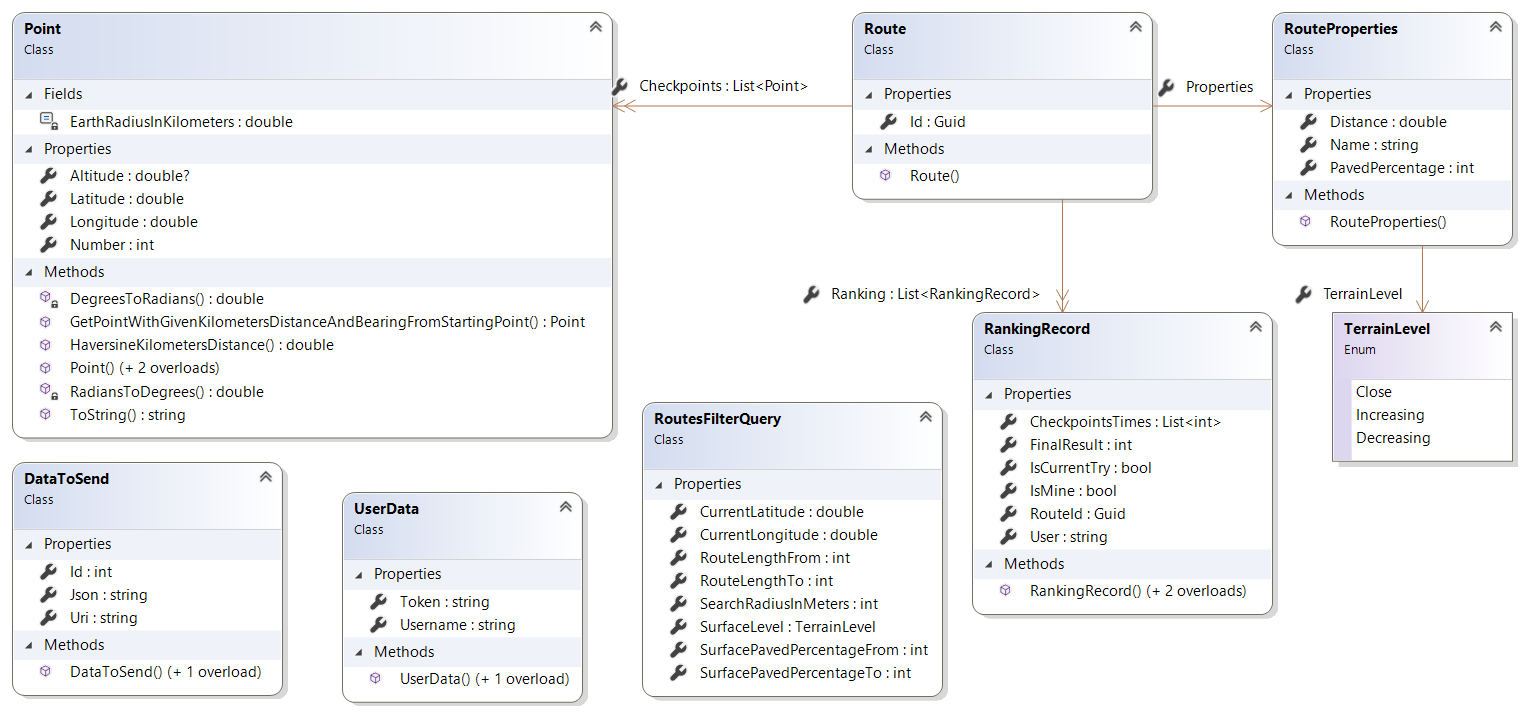
\includegraphics[width=\textwidth]{img/xamarin_model.png}
\caption{Diagram klas modelu danych aplikacji mobilnej [Opracowanie własne]}\label{image:xamarin_model}
\end{center}
\end{figure}
Ponad to model danych zawiera dwie dodatkowe klasy:
\begin{itemize}
\item{\textit{DataToSend}} - przechowuje dane w formacie JSON oraz adres URL. Pozwala podjąć ponowną, odłożoną w czasie próbę wysłania danych na serwer w przypadku gdy proces ten nie zakończy się sukcesem przy pierwszym podejściu.
\item{\textit{UserData}} - przechowuje dane o aktualnie zalogowanym użytkowniku: login użytkownika oraz token używany podczas komunikacji z serwerem.
\end{itemize}
\subsection{Aplikacja serwerowa}
Z racji podobieństwa do modelu danych zawartego w aplikacji mobilnej, który opisany został w rozdziale \ref{chap:model-mobilna}, w rozdziale niniejszym zostaną przybliżone jedynie nie omówione wcześniej aspekty. 

\begin{figure}[h]\label{fig:api_model}
\begin{center}
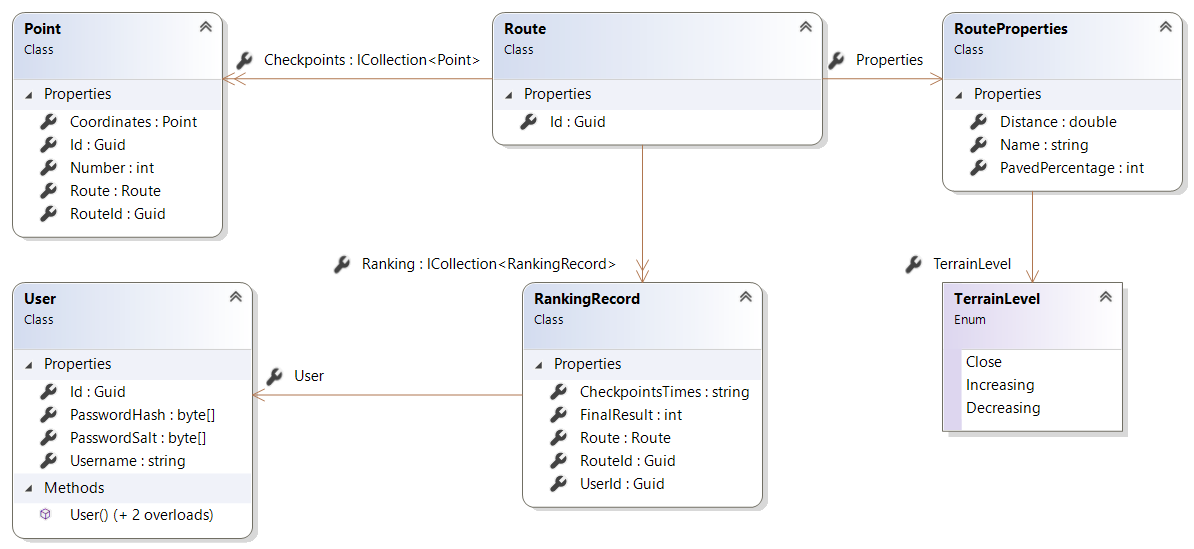
\includegraphics[width=\textwidth]{img/api_model.png}
\caption{Diagram klas modelu danych aplikacji serwerowej [Opracowanie własne]}\label{image:api_model}
\end{center}
\end{figure}

Jak widać na diagramie \ref{image:api_model} w modelu aplikacji serwerowej istnieje klasa \textit{User}. Reprezentuje ona konto użytkownika w systemie. Powiązanie tej klasy z klasą reprezentującą próbę na trasie, pozwala określić do którego z użytkowników należy konkretny wynik.

Współrzędne punktów trasy zapisywane przy użyciu typu danych \textit{Point}. Należy zaznaczyć, że nie jest to typ stworzony w ramach modelu danych, lecz należącą do przestrzeni nazw \textit{NetTopologySuite.Geometries}, występującą w środowisku .NET reprezentacją typu \textit{geography} istniejącego w systemie zarządzania bazą danych SQL Server. \textit{Geography} pozwala na przechowywanie współrzędnych geograficznych punktu (wraz z wysokością nad poziomem morza) w jednej kolumnie tabeli bazodanowej. \cite{geography-type}

\begin{figure}[h]
\begin{center}
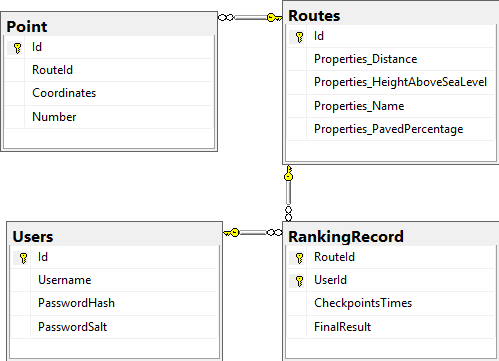
\includegraphics{img/er-diagram.png}
\caption{Diagram encji bazy danych [Opracowanie własne]}\label{image:db-structure}
\end{center}
\end{figure}

Zastosowanie mapowania obiektowo-relacyjnego pozwoliło na odwzorowanie modelu danych w formie bazy danych. Jej struktura została przedstawiona na rysunku \ref{image:db-structure}. Przed utworzeniem odpowiednich tabel konieczne było zdefiniowanie relacji pomiędzy polami tabel. Odpowiednią konfigurację umieszczono w klasie \textit{Context} znajdującej się w przestrzeni nazw \textit {Api.Entities} i przedstawiono na listingu \ref{listing:context}.

\begin{lstlisting}[caption={Konfiguracja mapowania relacyjno-obiektowego},label=listing:context]
protected override void OnModelCreating(
ModelBuilder modelBuilder)
{
    modelBuilder.Entity<Route>().HasMany(r => r.Checkpoints)
    	.WithOne(cp => cp.Route)
    	.HasForeignKey(cp => cp.RouteId);
    modelBuilder.Entity<Route>().OwnsOne(r => r.Properties);
    modelBuilder.Entity<Route>().HasMany(r => r.Ranking)
    	.WithOne(rr => rr.Route)
        .HasForeignKey(rr => rr.RouteId);

    modelBuilder.Entity<RankingRecord>().HasOne(rr => rr.User);
    modelBuilder.Entity<RankingRecord>()
    	.HasKey(rr => new { rr.RouteId, rr.UserId });

    base.OnModelCreating(modelBuilder);
}
\end{lstlisting}
Konfiguracja pozwoliła na utworzenie następujących relacji:
\begin{itemize}
\item{jeden do wielu pomiędzy tabelami reprezentującymi klasy \textit{Route}} oraz \textit{Point}
\item{jeden do wielu pomiędzy tabelami reprezentującymi klasy \textit{Route}} oraz \textit{RankingRecord}
\item{jeden do jednego pomiędzy tabelami reprezentującymi klasy \textit{RankingRecord} oraz \textit{User}}
\end{itemize}
Dzięki instrukcji z linii numer 7 dane z klas \textit{Route} oraz \textit{RouteProperties} zostały umieszczone w jednej tabeli. Pozwoliło to na uniknięcie łączenia tabel podczas pobierania danych. Typy wyliczeniowe nie wymagają osobnej tabeli i są przechowywane w postaci liczb, dlatego nie było potrzeby tworzenia dodatkowej struktury dla cechy \textit{poziom terenu}.

Warto zauważyć, że czasy osiągane na punktach kontrolnych są przechowywane jako łańcuch znaków (\textit{string}). Pozwoliło to uniknąć tworzenia dodatkowej tabeli i relacji jeden do wielu z tabelą reprezentującą klasę \textit{RankingRecord}. Mapowanie pomiędzy kolekcją a łańcuchem znaków odbywa się w klasie \textit{AutomapperConfig} znajdującej się w przestrzeni nazw \textit{Api.Mappers} i zostało przedstawione na listingu \ref{listing:collection-string-mapping}.
\begin{lstlisting}[caption={Mapowanie pomiedzy kolekcją a łańcuchem znaków},label=collection-string-mapping]
public static IMapper Initialize()
    => new MapperConfiguration(cfg =>
        {
         cfg.CreateMap<RankingRecord, RankingRecordDto>()
             .ForMember(dest => dest.CheckpointsTimes, opt =>
                    opt.MapFrom(src => src.CheckpointsTimes
                    .Split(" ", StringSplitOptions.None).Select(int.Parse)))
         cfg.CreateMap<RankingRecordDto, RankingRecord>()
             .ForMember(dest => dest.CheckpointsTimes,
                 opt => opt.MapFrom(src => 
                 string.Join(" ", src.CheckpointsTimes)))
        })
        .CreateMapper();
\end{lstlisting}

\section{Warstwa logiki biznesowej}
\section{Warstwa interfejsu użytkownika}